\documentclass[crop,tikz]{standalone}% 'crop' is the default for v1.0, before it was 'preview'
\usepackage{tikz,calc,pgfplots}
\usetikzlibrary{calc}
\begin{document}


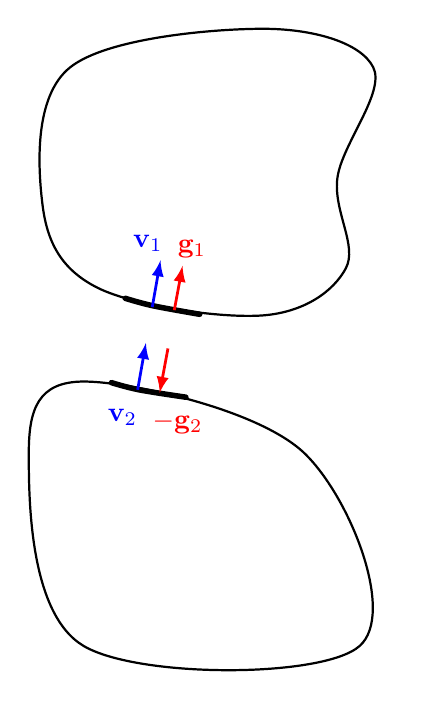
\begin{tikzpicture}[scale=0.7,rotate=0]

\begin{scope}[shift={(0.25,1.5)}]

 \draw [thick]  plot[smooth cycle, tension=.6] coordinates {(0,2) (0.5,4.5) (4,5.2) (6,4.5)  (5.35,2.5) (5.5,0.85) (4,0) (1,0.5) };
%\node[outer sep=0pt,thick] at (5.2,4.2) [minimum width=1.5cm, minimum height=1.5cm] {${S}$};
 
%\draw [thick,dashed, fill=white!70!black]  plot[smooth cycle,  tension=.6] coordinates {(1.5,2.8) (1.5,4) (2.5,4)  (2.5,3.2) };

%\node[outer sep=0pt,thick] at (2,3.5) [minimum width=1.5cm, minimum height=1.5cm] {$o$};
 
 
% \draw [line width=2pt,black,cap=round]  plot[smooth, tension=.6] coordinates { (3.25,5.175) (4,5.2) (4.75,5.15) };  
% \node[outer sep=0pt,thick] at (4,5.5) [minimum width=1.5cm, minimum height=1.5cm] {$a$};
% 
 \draw [line width=2pt,black,cap=round]  plot[smooth, tension=.6] coordinates { (2.85,0.02) (2,0.175) (1.5,0.31) };  
% \node[outer sep=0pt,thick] at (3,0.35) [minimum width=1.5cm, minimum height=1.5cm] {$1$};
 
 \end{scope}
 
%\draw [line width=1pt,black,cap=round]  plot[smooth, tension=.6] coordinates { (2.85,0.016) ($(2.85,0.02) + (0.25,1.5)$) };  
%\draw [line width=1pt,black,cap=round]  plot[smooth, tension=.6] coordinates { (1.5,0.31)  ($(1.5,0.31) + (0.25,1.5)$) };  
%\node[outer sep=0pt,thick] at ($(2,0.175)+ (0.3,0.65)$) [minimum width=1.5cm, minimum height=1.5cm] {${I_1}$}; 


\draw [thick]  plot[smooth cycle, tension=.6] coordinates {(0,-1) (1,-4.5) (6,-4.5) (5,-1) (1,0.3) };
%\node[outer sep=0pt,thick] at (5.5,-4) [minimum width=1.5cm, minimum height=1.5cm] {${R}$};

\draw [line width=2pt,cap=round]  plot[smooth, tension=.6] coordinates { (2.85,0.016) (2,0.15) (1.5,0.28) };  
\draw [line width=1pt,red,latex-]  plot[smooth, tension=.6] coordinates { (2.375,0.095)  (2.525,0.9) };   
 \begin{scope}[shift={(0.36,1.5)}]
 \draw [line width=1pt,red,-latex]  plot[smooth, tension=.6] coordinates { (2.28,0.095)  (2.43,0.9) };   
  \node[outer sep=0pt,thick] at (2.6,1.2) [minimum width=1.5cm, minimum height=1.5cm] {${\color{red}\mathbf{g}_1}$}; 
 \end{scope}  
  \node[outer sep=0pt,thick] at (2.7,-0.45) [minimum width=1.5cm, minimum height=1.5cm] {${\color{red}-\mathbf{g}_2}$}; 
 
\draw [line width=1pt,blue,-latex]  plot[smooth, tension=.6] coordinates { (1.975,0.15)  (2.125,1) };   
\begin{scope}[shift={(0.36,1.5)}]
\draw [line width=1pt,blue,-latex]  plot[smooth, tension=.6] coordinates { (1.88,0.15)  (2.03,1) };   
  \node[outer sep=0pt,thick] at (1.8,1.3) [minimum width=1.5cm, minimum height=1.5cm] {${\color{blue}\mathbf{v}_1}$}; 
\end{scope}  
    \node[outer sep=0pt,thick] at (1.7,-0.35) [minimum width=1.5cm, minimum height=1.5cm] {${\color{blue}\mathbf{v}_2}$}; 
 \end{tikzpicture}
\end{document}